\documentclass[11pt]{book}
\usepackage{amsmath,amssymb,amsthm}
\usepackage{makeidx}
\usepackage{verbatim}
\usepackage{listings}
\usepackage{color}
\usepackage{subfigure}
\usepackage[final]{graphicx}

\graphicspath{{eps/}}

\definecolor{tan}{rgb}{0.93,0.87,0.80}

\oddsidemargin 0.25in
\evensidemargin .025in
\topmargin 0.5in

\makeindex

\numberwithin{equation}{section}
\renewcommand{\labelenumi}{\alph{enumi}}

\bibliographystyle{plain}

\newcommand{\N}{\mathbb{N}}
\newcommand{\impl}{\rightarrow}

\newtheorem*{claim}{\textit{Claim}}
\newtheorem*{proofofclaim}{\textit{Proof of Claim}}
\newtheorem{thm}{Theorem}[section]
\newtheorem{cor}[thm]{Corollary}
\newtheorem{lem}[thm]{Lemma}
\newtheorem{prop}[thm]{Proposition}
\newtheorem{note}[thm]{\textit{Note}}
\theoremstyle{definition}
\newtheorem{dfn}[thm]{Definition}
\newtheorem{examp}[thm]{Example}

\lstset{ %
language=C++,                % choose the language of the code
basicstyle=\footnotesize,       % the size of the fonts that are used for the code
numbers=left,                   % where to put the line-numbers
numberstyle=\footnotesize,      % the size of the fonts that are used for the line-numbers
%stepnumber=2,                   % the step between two line-numbers. If it's 1 each line will be numbered
%numbersep=5pt,                  % how far the line-numbers are from the code
backgroundcolor=\color{tan},  % choose the background color. You must add \usepackage{color}
%showspaces=false,               % show spaces adding particular underscores
%showstringspaces=false,         % underline spaces within strings
%showtabs=false,                 % show tabs within strings adding particular underscores
frame=single,                   % adds a frame around the code
tabsize=2,                      % sets default tabsize to 2 spaces
captionpos=b,                   % sets the caption-position to bottom
breaklines=true,                % sets automatic line breaking
breakatwhitespace=false,        % sets if automatic breaks should only happen at whitespace
escapeinside={\%*}{*)}          % if you want to add a comment within your code
}


%\typein [\files]{Enter file names to process, (chap1,chap2 ...), or `all' to process all files:}
%\def\all{all}
%\ifx\files\all \typeout{Including all files.} \else \typeout{Including only \files.} \includeonly{\files} \fi

\begin{document}
  \begin{titlepage}
	\begin{center}
		\vspace*{1in}
		{\LARGE Basics of Computational Image Analysis\\}
		{\large With examples in Matlab andC++}
		\par
		\vspace{0.75in}
		{\large Chad Rempp}
		\par
		\vfill
		\vspace{0.25in}
		%Something
		\par
		\vspace{0.25in}
		%Something
		\par
		\vspace{0.25in}
		\today
	\end{center}
\end{titlepage}

%\newpage
%\section*{Acknowledgments}
%I would like to thank no one!

  
  \pagestyle{plain}
  \tableofcontents
%  \listoftables
%  \listoffigures
  
  \chapter{Foundations}
	In the development of image analysis there are many theorems that depend on real and complex analysis. This section presents the required material but does not prove any theorems or explain them in detail. For a deeper understanding of these concepts see the cited references.
	
\section{Topology and Measures}\label{measures}
	These come from Rudin \cite{rudin_1}.
\begin{comment}
Introduce topology.
\begin{dfn}\index{topology}
	A collection $\tau$ of subsets of a set $X$ is a \emph{topology} in $X$ if $\tau$ has the following properties:
	\begin{enumerate}
	\item $\emptyset\in\tau$ and $X\in\tau$.
	\item if $V_i\in\tau$ for $i=1,\ldots,n$, then $V_1\cap\cdots\cap V_n\in\tau$.
	\item If $\{V_\alpha\}$ is an arbitrary collection of members of $\tau$, then $\bigcup_\alpha V_\alpha\in\tau$.
	\end{enumerate}
\end{dfn}
\begin{dfn}\index{$\sigma$-algegra}
	A collection $\mathfrak{M}$ of subsets of $X$ is a \emph{$\sigma$-algegra} if $\mathfrak{M}$ has the following properties in $X$:
	\begin{enumerate}
	\item $X\in\mathfrak{M}$.
	\item If $A\in\mathfrak{M}$ then $A^C\in\mathfrak{M}$ where $A^C$ is the complement of $A$ in $X$.
	\item If $A=\cup_{n=1}^\infty A_n$ for $n=1,2,\ldots$ and $A\in\mathfrak{M}$ then $A\in\mathfrak{M}$
	\end{enumerate}
\end{dfn}
\end{comment}
	Measure theory provides the notion of length, area and volume of sets. This is necessary for the formal definitions of integrals.
\begin{dfn}\index{measure!measurable space}
	If $\mathfrak{M}$ is a $\sigma$-algegra in $X$, then $X$ is a \emph{measurable space}. The members of $\mathfrak{M}$ are the \emph{measurable sets} in $X$.
\end{dfn}
\begin{dfn}\index{measure!measurable}
	If $X$ is a measurable space, $Y$ is a topological space and $f:X\rightarrow Y$ then $f$ is \emph{measurable} if $f^{-1}(V)$ is measurable in $X$ for every open set $V$ in $Y$.
\end{dfn}
\begin{dfn}\index{countably additive}
	A function $\mu$ defined on a $\sigma$-algebra $\mathfrak{M}$ is \emph{countably additive} means that if $\{A_i\}$ is a disjoint countable collection of members of $\mathfrak{M}$ then
	\begin{equation*}
		\mu(\bigcup_{i=1}^\infty A_i)=\sum_{i=1}^\infty\mu(A_i).
	\end{equation*}
\end{dfn}
\begin{dfn}\index{measure!positive measure}\index{measure!measure}
	A \emph{positive measure} (measure) is a function $\mu$, defined on a $\sigma$-algebra $\mathfrak{M}$, whose range is in $[0,\infty]$ and which is countably additive.
\end{dfn}
\begin{dfn}\index{measure!measure space}
	A \emph{measure space} is a measurable space which has a positive measure defined on the $\sigma$-algebra of its measurable sets.
\end{dfn}
\begin{comment}
A set is Lebesque measurable if it can be assigned a volume.
\begin{dfn}\index{Lebesgue measurable}
	See \cite{rudin_1} p. 53
\end{dfn}
\begin{dfn}\index{Lebesgue measure}
	See \cite{rudin_1} p. 53
\end{dfn}

\section{$L^p$ Spaces}
\begin{dfn}\index{$L^p$ norm}
	If $X$ is an arbitrary measure space with positve measure $\mu$
\end
\begin{dfn}\index{$L^p$ norm}
	
\end
\end{comment}

%-----L^p Spaces----------------------------------------------------------------
\section{$\mathbf{L}^p$ Spaces}

A $\mathbf{L^p}$ space is a normed vector space(?).
\begin{dfn}\index{$\mathbf{L}^p$-norm}
	Let $(X,\mathfrak{M},\mu)$ be a measure space and $0<p<\infty$. The $\mathbf{L}^p$-norm of a function $f:X\rightarrow\mathbb{R}$ is defined as:
	\begin{equation*}
		\|f\|_p=\left(\int_X|f|^pd\mu\right)^{1/p}
	\end{equation*}
\end{dfn}

\begin{dfn}[$\mathbf{L}^p$ Space]\cite{jones_1}
	
	Let $1\leq p<\infty$ and $f:X\rightarrow\mathbb{R}$ then the set of functions:
	\begin{equation*}
		\mathbf{L}^p=\{f:\mathbf{L^p}\int_X|f|^p d\mu<\infty\}
	\end{equation*}
	is a vector space called the \emph{$\mathbf{L}^p$ space}.
\end{dfn}

\begin{comment}
The following properties are valid. (prove these)
\begin{enumerate}
\item $0\leq\|f\|_P<\infty$
\item $\|f\|_P=0\text{ iff }f=0$
\item $\|cf\|_P=|c| \|f\|_P\text{ if }c\in\mathbb{R}$
\item $\|f+g\|_P\leq\|f\|_P+\|g\|_P$
\end{enumerate}
\end{comment}


  \chapter{The Convolution and Correlation}
	One of the most important concepts in image analysis is convolution. The convolution is a transform that takes two functions and returns a different function. This new function has been created by essentially smearing one of the functions over the other combining their magnitude at every point. Figure \ref{fig_convolution} shows how this is done.

\section{One-Dimensional Convolution}

	\begin{dfn}\index{convolution!one-dimensional}
		Let $f$ and $g$ belong to $L^1(\mathbb{R})$. The \emph{convolution}, $f*g$ defined as:
		\begin{equation}\label{def_convolve_1D}
			(f*g)(x)=\int_{-\infty}^\infty f(x-\tau)g(\tau)d\tau
		\end{equation}
	\end{dfn}

	In the context of image analysis we are dealing with real-valued functions that are generally bounded (by intensity such as 0 to 255). So these functions behave nicely and therefore we can assume the covolution exists. For more information on the existance of the convolution see Yeh \cite{yeh_1}.

	\begin{figure}[!htb]
			\centering
			\subfigure[$f(x)$]{
				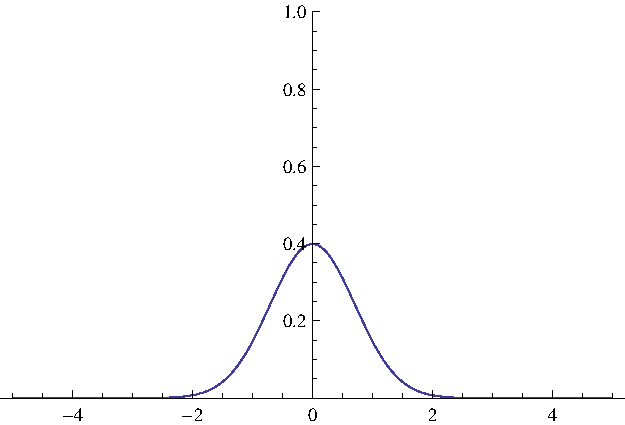
\includegraphics[width=2in]{graph_01}}
			\subfigure[$g(x)$]{
				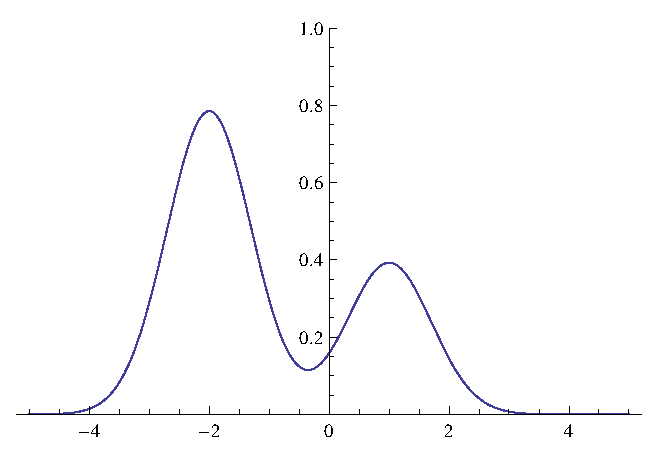
\includegraphics[width=2in]{graph_02}}
			\subfigure[$f(x-2)g(x)$]{
				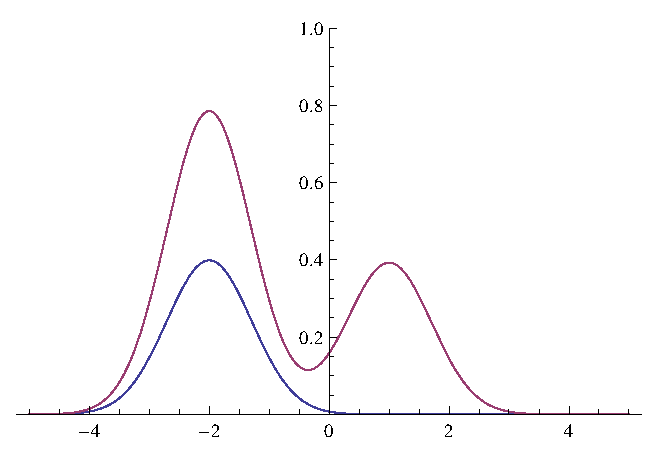
\includegraphics[width=2in]{graph_03}}
			\subfigure[$f(x-1)g(x)$]{
				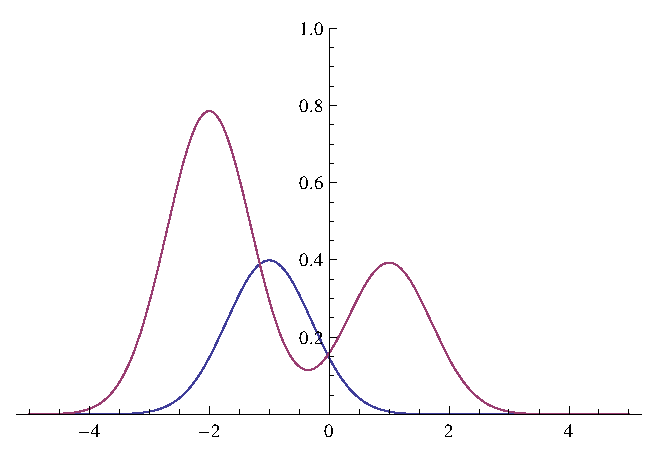
\includegraphics[width=2in]{graph_04}}
			\subfigure[$f(x-0)g(x)$]{
				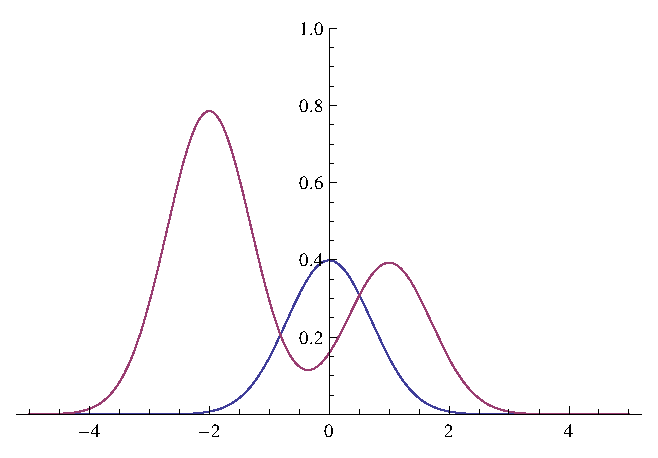
\includegraphics[width=2in]{graph_05}}
			\subfigure[$f(x+1)g(x)$]{
				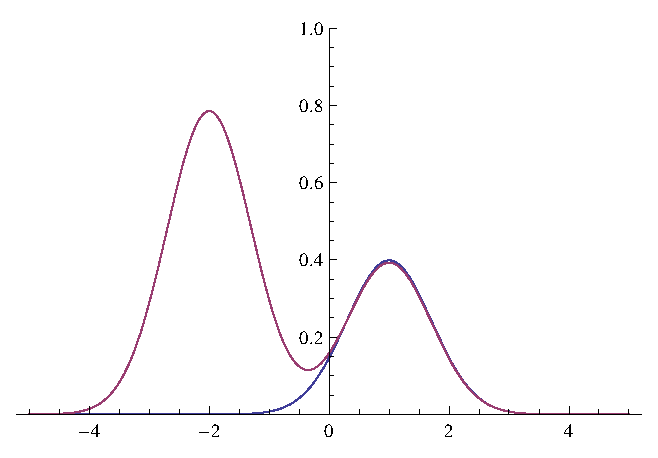
\includegraphics[width=2in]{graph_06}}
			\subfigure[$f(x+2)g(x)$]{
				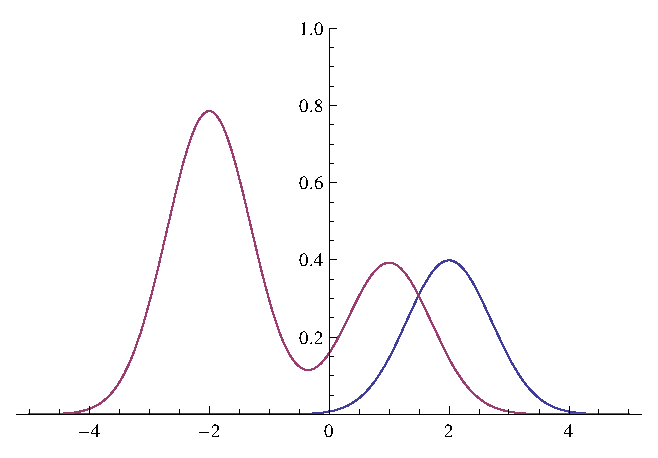
\includegraphics[width=2in]{graph_07}}
			\subfigure[$f*g$]{
				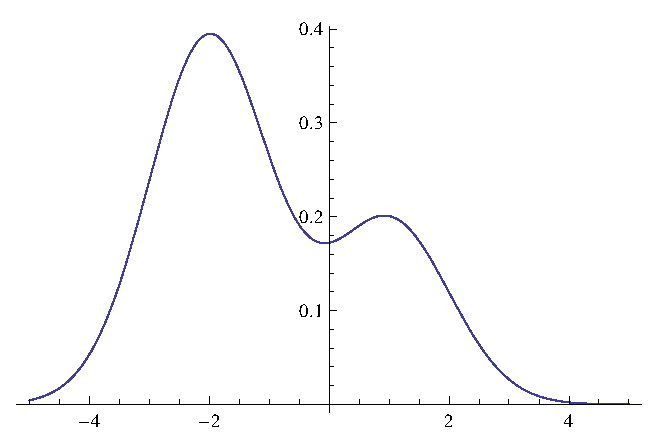
\includegraphics[width=2in]{graph_08}}
			\caption{One-dimensional convolution example}
			\label{fig_convolution}
	\end{figure}
	\clearpage
	
	The convolution has many properties that are useful. 
	\begin{prop}
		The convolution has the following properties (prove).
		\begin{enumerate}
		\item $f*g=g*f$ (commutative)
		\item $f*(g*h)=(f*g)*h$ (associative)
		\item $f*(g+h)=(f*g)+(f*h)$ (distributive)
		\item $a(f*g)=(af*g)=(f*ag)s$ for $a\in\mathbb{R}$ (associativity with scalar multiplication)
		\end{enumerate}
	\end{prop}
	\begin{proof}\hspace{10mm}
		\begin{enumerate}
		\item Substitute $\kappa=x-\tau$, $d\kappa=-d\tau$ into the defintion of convolution so \mbox{$(f*g)(x)=-\int_{\infty}^{-\infty}f(\kappa)g(x-\kappa)d\kappa$}. Switching the limits of integration and the order of $f$ and $g$ we have \mbox{$(f*g)(x)=\int_{-\infty}^\infty g(x-\kappa)f(\kappa)d\kappa$}. Rename the variable of integration $\kappa$ back to $\tau$ (this rename doesn't change anything) and we get \mbox{$(f*g)(x)=\int_{-\infty}^\infty g(x-\tau)f(\tau)d\tau=(g*f)(x)$}
		\item Using the defintion
			\begin{equation*}\begin{array}{rl}
				(f*(g*h))(x)&=\int_{-\infty}^\infty f(x-\tau)(g*h)(\tau)d\tau\\
				&=\int_{-\infty}^\infty f(x-\tau)\left[ \int_{-\infty}^\infty g(\tau-\kappa)h(\kappa)d\kappa\right]d\tau\\
				&=\int_{-\infty}^\infty\int_{-\infty}^\infty f(x-\tau)g(\tau-\kappa)h(\kappa)d\kappa d\tau.
			\end{array}\end{equation*}
			By Fubini's theorem we can switch the order of integration so
			\begin{equation*}\begin{array}{rl}
				(f*(g*h))(x)&=\int_{-\infty}^\infty\int_{-\infty}^\infty f(x-\tau)g(\tau-\kappa)h(\kappa)d\tau d\kappa\\
				&=\int_{-\infty}^\infty f(x-\tau)\left[\int_{-\infty}^\infty g(\tau-\kappa)h(\kappa)d\tau\right]d\kappa.
			\end{array}\end{equation*}
			Since we are working in a translation invarient metric we have
			\begin{equation*}\begin{array}{rl}
				(f*(g*h))(x)&=\int_{-\infty}^\infty f(x-\tau)\int_{-\infty}^\infty[g((\tau+\kappa)-\kappa)h(x-(\tau+\kappa))d\tau]d\kappa\\
				&=\int_{-\infty}^\infty f(x-\tau)\int_{-\infty}^\infty[g(\tau)h((x-\kappa)-\tau))d\tau]d\kappa\\
				&=\int_{-\infty}^\infty f(x-\tau)(g*h)(x-\kappa)d\kappa\\
				&=((f*g)*h)(x).
			\end{array}\end{equation*}
		\item
			\begin{equation*}\begin{array}{rl}
				(f*(g+h))(x)&=\int_{-\infty}^\infty f(x-\tau)(g(\tau)+h(\tau))d\tau\\
				&=\int_{-\infty}^\infty f(x-\tau)g(\tau)+f(x-\tau)h(\tau))d\tau\\
				&=\int_{-\infty}^\infty f(x-\tau)g(\tau)+\int_{-\infty}^\infty f(x-\tau)h(\tau))d\tau\\
				&=(f*g)(x)+(f*h)(x).
			\end{array}\end{equation*}
		\item
			\begin{equation*}\begin{array}{rl}
				a(f*g)(x)&=a\int_{-\infty}^\infty f(x-\tau)g(\tau)d\tau\\
				&=\int_{-\infty}^\infty af(x-\tau)g(\tau)d\tau\\
				&=(af*h)(x).
			\end{array}\end{equation*}
			The other equality is proved exactly the same way.
		\end{enumerate}
	\end{proof}
	
	Differentiation.
	\begin{equation*}\index{convolution!derivative 1D}
		\frac{d}{dx}(f*g)=(\frac{df}{dx}*g)(x)=(f*\frac{dg}{dx}g)(x)
	\end{equation*}
	
	
\section{Two-Dimensional Convolution}
	In two dimensions:
	\begin{dfn}\index{convolution!two-dimensional}
		Let $f$ and $g$ belong to $L^2{\mathbb{R^2}}$. The convolution, $(f*g)$ defined as:
		\begin{equation}\label{def_convolve_2D}
			(f*g)(x,y)=\int_{-\infty}^\infty\int_{-\infty}^\infty f(x-\tau,y-\kappa)g(\tau,\kappa)d\tau d\kappa
		\end{equation}
	\end{dfn}
	
	Differentiation in two variables.
	\begin{equation*}\index{convolution!derivative 2D}
		\frac{\partial}{\partial x}(f*g)=\frac{\partial f}{\partial x}*g=f*\frac{\partial g}{\partial x}
	\end{equation*}
	\begin{equation*}
		\frac{\partial}{\partial y}(f*g)=\frac{\partial f}{\partial y}*g=f*\frac{\partial g}{\partial y}
	\end{equation*}

\section{Discrete Convolution}
	We will only examine the two dimensional case.
	\begin{dfn}
		Let $f$ and $g$ be functions ...?
		\begin{equation*}\index{convolution!two-dimensional discrete}
			(f\otimes g)(x,y)=\sum_{i=0}^{M-1}\sum_{j=0}^{N-1}f(i-x,j-y)g(i,j).
		\end{equation*}
	\end{dfn}

\section{Convolution Implementation}

	\lstinputlisting{test.c}

\section{One-Dimensional Correlation}
	Correlation
	\begin{dfn}
		
	\end{dfn}

  
  \appendix
  \chapter{Test appendix}

Test test


  \bibliography{bibliography}
  
  \printindex
\end{document}





